
\subsection{Что это?}

\frame{
    \frametitle{Что такое <<нечеткие дубликаты>>}

    %\insertsectionhead

    \begin{tabular}{ccccc}
        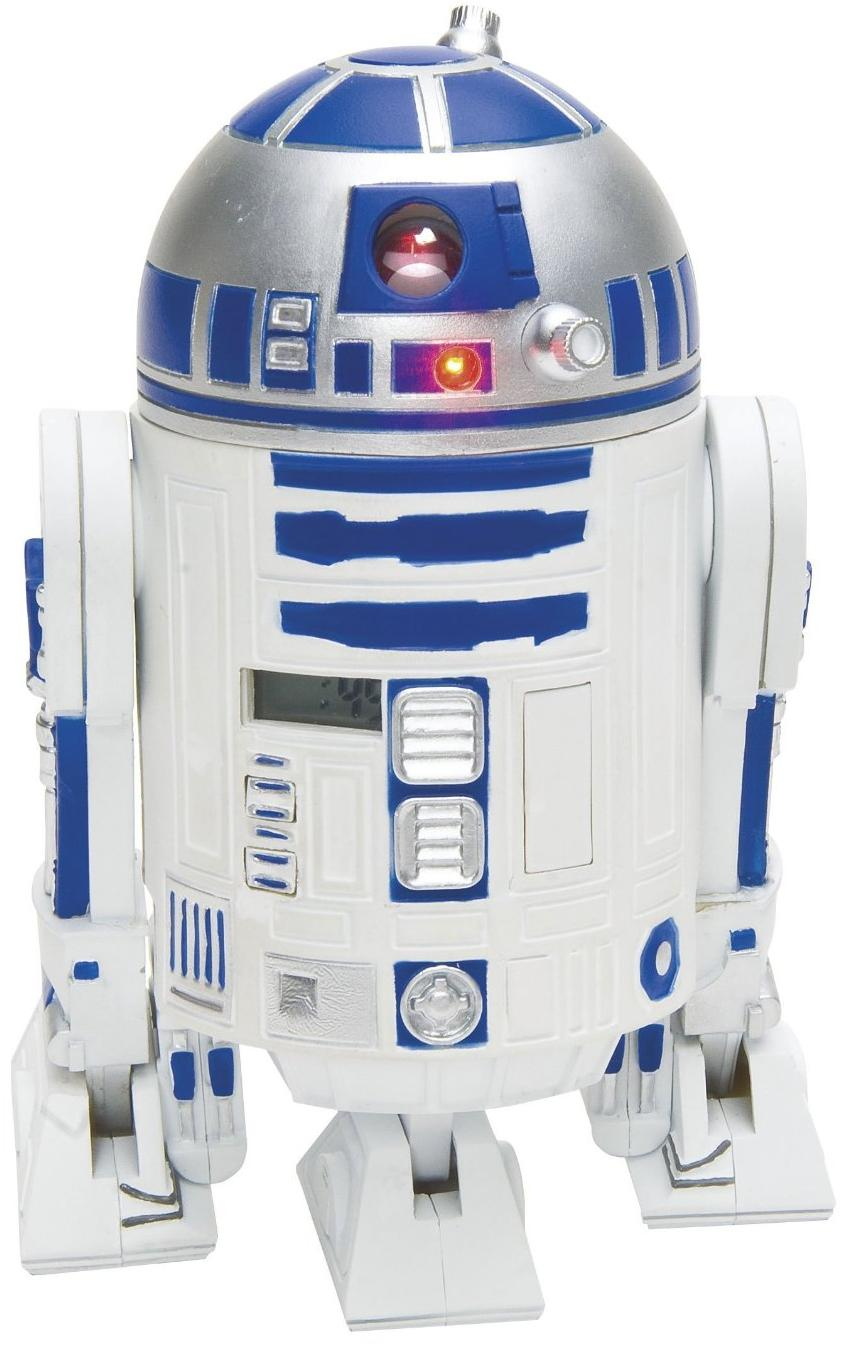
\includegraphics[height=4cm]{./img/near-dublicate-3-1.jpg}
        &
        %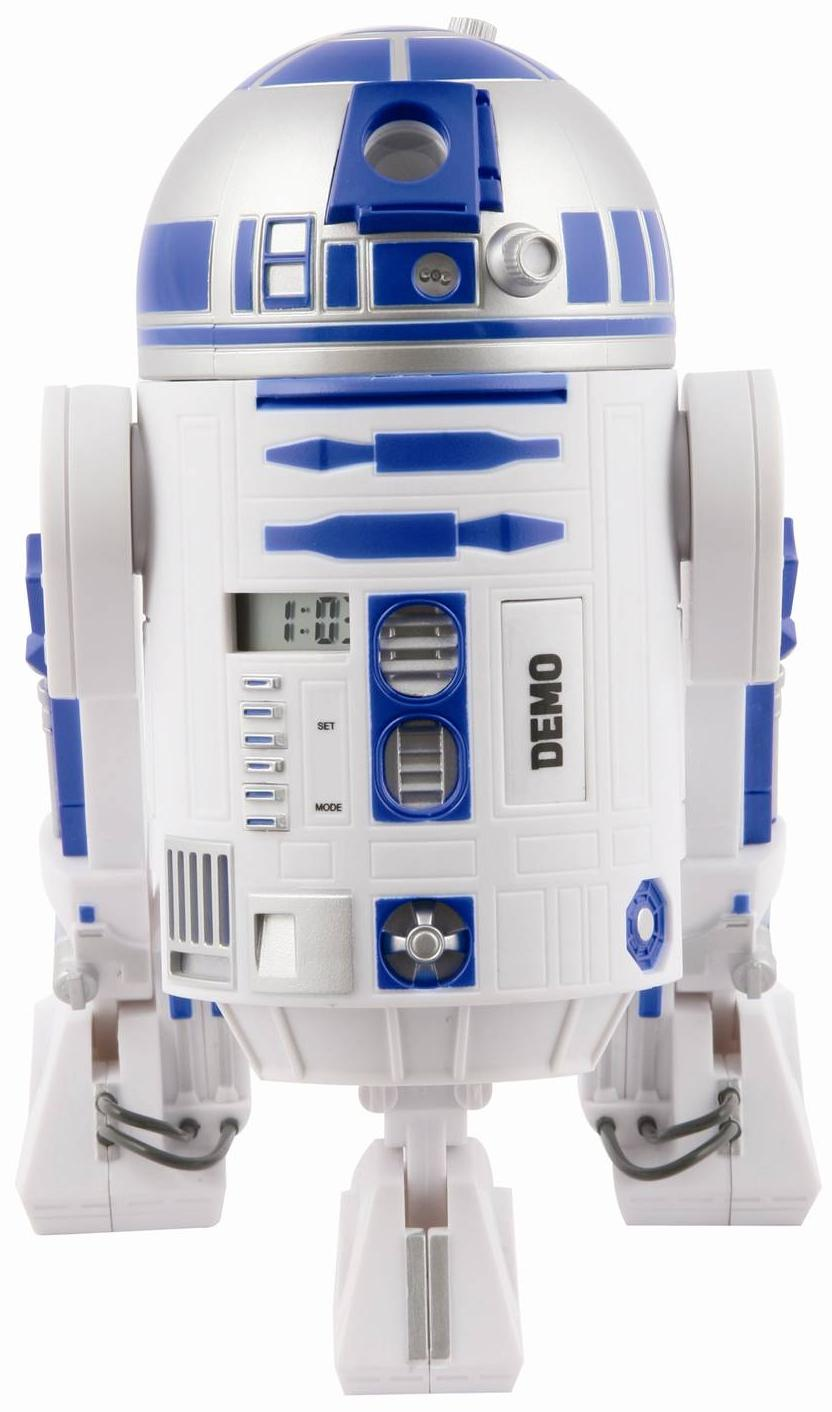
\includegraphics[height=4cm]{./img/near-dublicate-3-2.jpg}
        &
        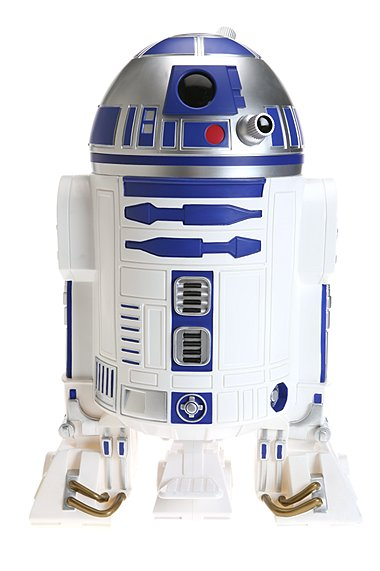
\includegraphics[height=4cm]{./img/near-dublicate-3-3.jpg}
        &
        %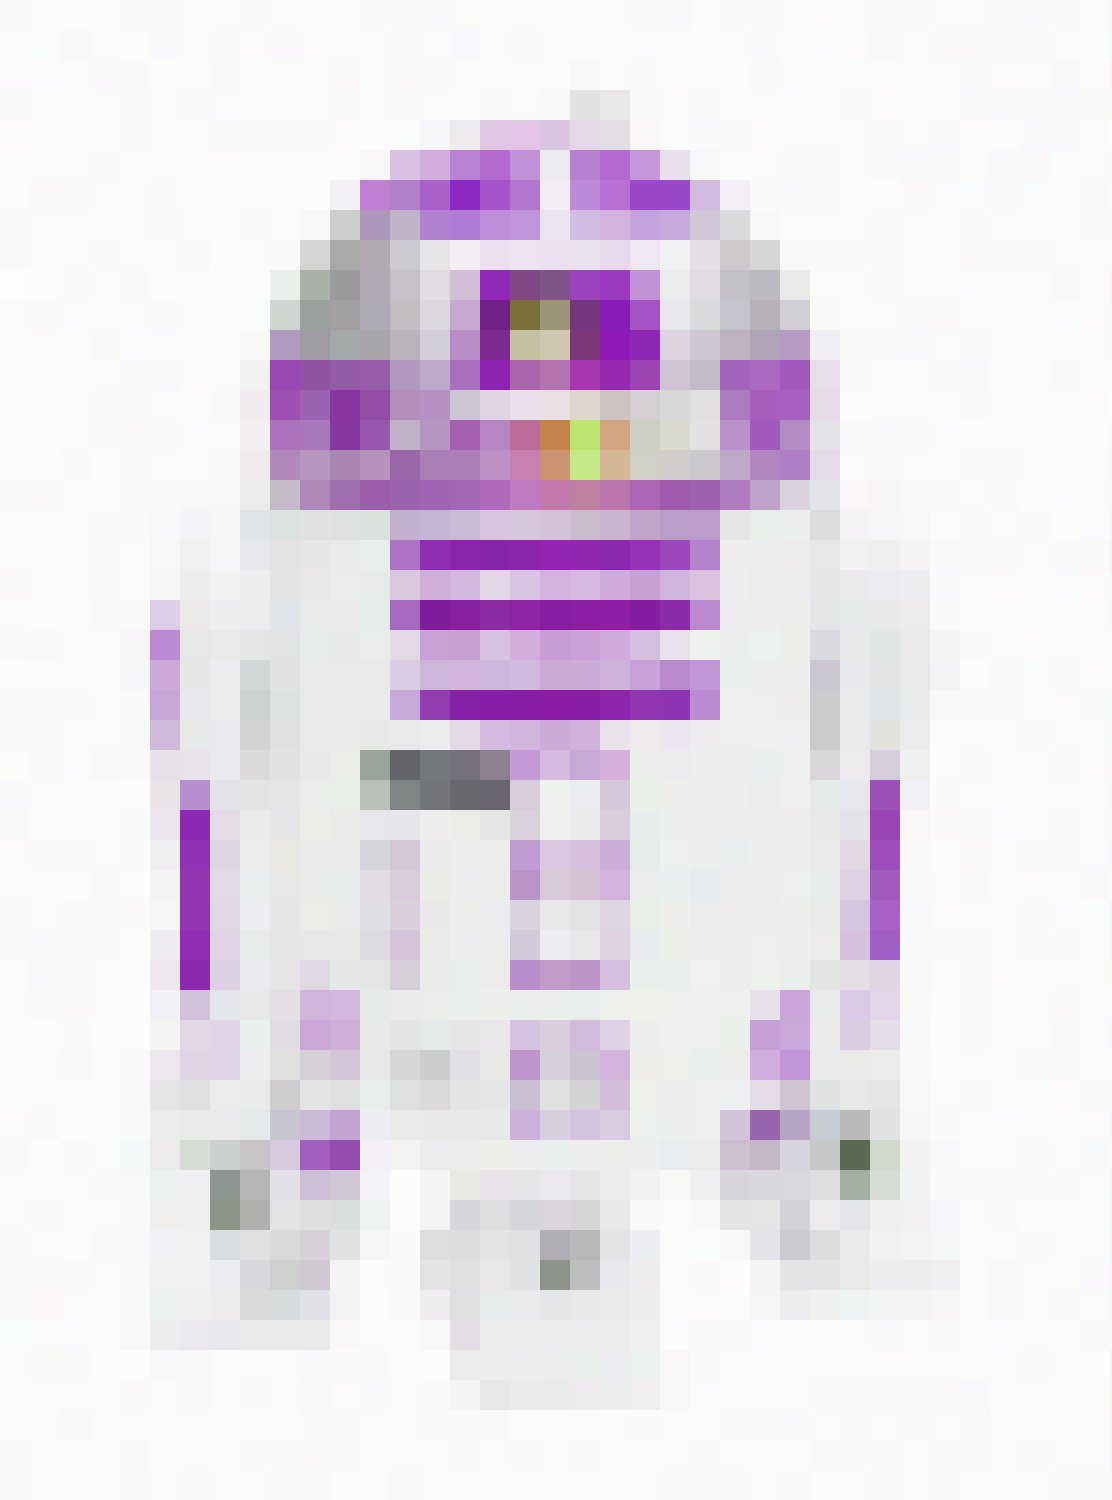
\includegraphics[height=4cm]{./img/near-dublicate-3-4.jpg}
        &
        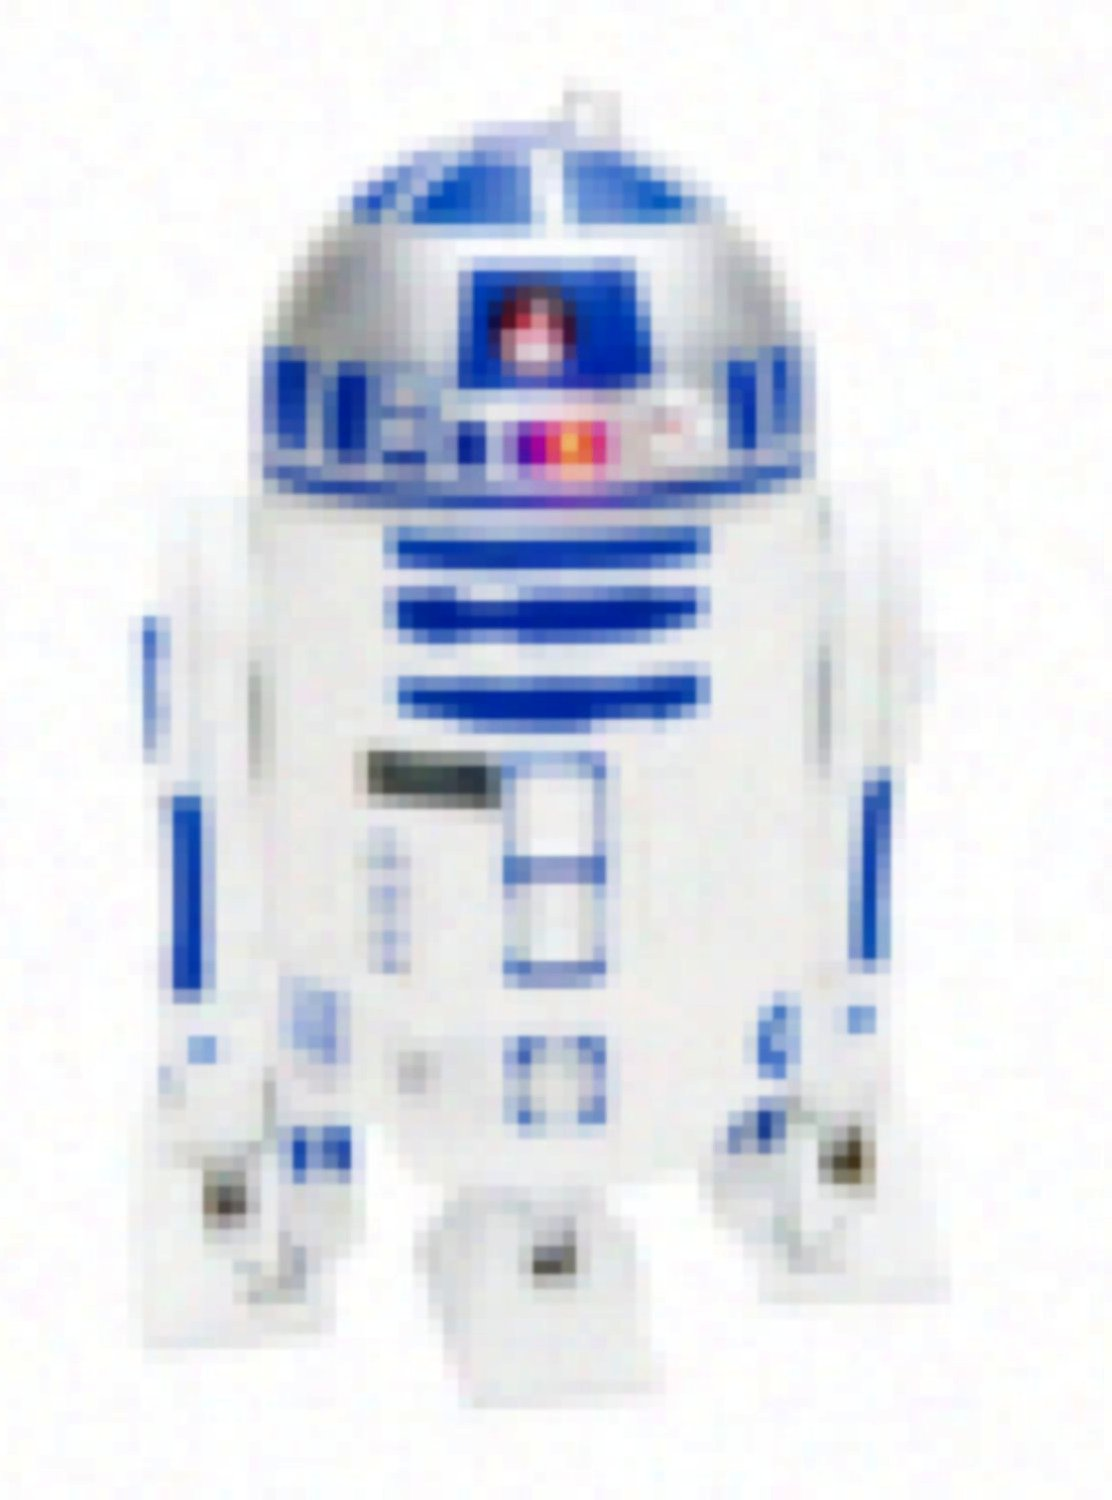
\includegraphics[height=4cm]{./img/near-dublicate-3-5.jpg}
        \\
        {\small оригинал}
        &
        %естественный дубликат
        &
        {\footnotesize естественный дубликат}
        &
        %искусственный дубликат
        &
        {\footnotesize искусственный дубликат}
        \\
    \end{tabular}
}
